% THIS IS SIGPROC-SP.TEX - VERSION 3.1
% WORKS WITH V3.2SP OF ACM_PROC_ARTICLE-SP.CLS
% APRIL 2009
%
% It is an example file showing how to use the 'acm_proc_article-sp.cls' V3.2SP
% LaTeX2e document class file for Conference Proceedings submissions.
% ----------------------------------------------------------------------------------------------------------------
% This .tex file (and associated .cls V3.2SP) *DOES NOT* produce:
%       1) The Permission Statement
%       2) The Conference (location) Info information
%       3) The Copyright Line with ACM data
%       4) Page numbering
% ---------------------------------------------------------------------------------------------------------------
% It is an example which *does* use the .bib file (from which the .bbl file
% is produced).
% REMEMBER HOWEVER: After having produced the .bbl file,
% and prior to final submission,
% you need to 'insert'  your .bbl file into your source .tex file so as to provide
% ONE 'self-contained' source file.
%
% Questions regarding SIGS should be sent to
% Adrienne Griscti ---> griscti@acm.org
%
% Questions/suggestions regarding the guidelines, .tex and .cls files, etc. to
% Gerald Murray ---> murray@hq.acm.org
%
% For tracking purposes - this is V3.1SP - APRIL 2009

\documentclass{acm_proc_article-sp}
\begin{document}

\title{PBECV: a fast resume extracting framework based on writing style recognition}
\subtitle{Resume extraction}
\titlenote{A full version of this paper is available}
\textit{}

%
% You need the command \numberofauthors to handle the 'placement
% and alignment' of the authors beneath the title.
%
% For aesthetic reasons, we recommend 'three authors at a time'
% i.e. three 'name/affiliation blocks' be placed beneath the title.
%
% NOTE: You are NOT restricted in how many 'rows' of
% "name/affiliations" may appear. We just ask that you restrict
% the number of 'columns' to three.
%
% Because of the available 'opening page real-estate'
% we ask you to refrain from putting more than six authors
% (two rows with three columns) beneath the article title.
% More than six makes the first-page appear very cluttered indeed.
%
% Use the \alignauthor commands to handle the names
% and affiliations for an 'aesthetic maximum' of six authors.
% Add names, affiliations, addresses for
% the seventh etc. author(s) as the argument for the
% \additionalauthors command.
% These 'additional authors' will be output/set for you
% without further effort on your part as the last section in
% the body of your article BEFORE References or any Appendices.

%\numberofauthors{8} %  in this sample file, there are a *total*
% of EIGHT authors. SIX appear on the 'first-page' (for formatting
% reasons) and the remaining two appear in the \additionalauthors section.
%
%\author{
% You can go ahead and credit any number of authors here,
% e.g. one 'row of three' or two rows (consisting of one row of three
% and a second row of one, two or three).
%
% The command \alignauthor (no curly braces needed) should
% precede each author name, affiliation/snail-mail address and
% e-mail address. Additionally, tag each line of
% affiliation/address with \affaddr, and tag the
% e-mail address with \email.
%
% 1st. author
%\alignauthor
%Chen Jie\\
%     \affaddr{Beijing Institute of Technology}\\
%       \affaddr{ 5 South Zhongguancun Street }\\
%       \affaddr{Haidian District, Beijing}\\
%       \email{sonyfe25cp@gmail.com}
% 2nd. author
%\alignauthor
%Zhendong Niu\\
%         \affaddr{Beijing Institute of Technology}\\
%       \affaddr{ 5 South Zhongguancun Street }\\
%       \affaddr{Haidian District, Beijing}\\
%       \email{zniu@bit.edu.cn}
%3rd.author
%\alignauthor
%Hongping Fu\\
%         \affaddr{Beijing Institute of Technology}\\
%       \affaddr{ 5 South Zhongguancun Street }\\
%       \affaddr{Haidian District, Beijing}\\
%       \email{fhongping@bit.edu.cn}
%}

\maketitle
\begin{abstract}


In the information age, companies receive thousands of resumes from job seekers everyday. 
Most of resumes are wrote in different format, including font size, font color and cells. %, except those follow the same template.
%For resumes adopt the common template file, they can be accurate interpred with the specific parser, but how to control the transfer efficiency?
%Since these resumes are different, it's difficult to structure these data.
As a result, it's difficult to structure these data with a general extracting method. 
%In this paper, we propose a fast approach to extract the resume information from text file which drop the structure information like the font size and table constraint.
In this paper, we propose PBECV to extract the resume information from text file without format information. 
Our appoach consider the writing style of each resume as the latent pattern, which help to segment resume text into different blocks and easy to parse. 
%The aim of this application scene is to build the baseline of resume extraction.
%The experiments on the real word data, our approach can reach the proformance of those alg used the structure information and the alg is fastest.
The experimental results on the real world data-set of millions of resumes show that our approach can reach the performance of algorithms that trained with the structure information and the proposed approach's algorithm complexity is O(n).

\end{abstract}

% A category with the (minimum) three required fields
%\category{H.4}{Information Systems Applications}{Miscellaneous}
%A category including the fourth, optional field follows...
%\category{D.2.8}{Software Engineering}{Metrics}[complexity measures, performance measures]

\terms{Algorithms, Design, Experimentation}

\keywords{resume information extraction, structure resume data}

\section{Introduction}

%In the information age, head-hunting companies collect millions of resumes. 
In the information age, head-hunting companies collect millions of resumes to occupy more market share.
%However, these resumes are not wrote with the standard format.
However, most of resumes are not wrote with the standard format or follow some special template file.
In order to improve the success rate of recommending some person to fit the requirements of employer, those resumes should be parsed exactly and detailed.
This helps headhunters to easily and quickly search for the right candidate.
The challenge is how to analysis the different kinds of resume to get the detailed information.

However, resumes are easier to structure than other texts, such as news. 
Different people have different writing style about personal resume, but the content of these work all around the same topic, their personal information, which contains contacts, educations, work experimences and so on.
%As a result of this, resumes can be segmented by servel groups.
As a result of this, resumes can be segmented into servel groups, which is one of the basic ideas to solve the problem.
In other words, resumes share the document-level hierarchical contextual structure \cite{maheshwari2010approach}.

There are three main methods to deal with resumes in the practical engineering. 
Firstly, since many engineers has the knowledge background about how to parse a web page based on the DOM structure, they treate the resume text as a web page to extracte the details. 
In particular, some big recruiting platform like Monster\footnote{http://www.monster.com/} and LinkedIn\footnote{http://www.linkedin.com} provide many beautiful template which make many resumes follow them.
This kind of resumes can be parsed through special template file or regex rules.
%The advantage is very high accuracy, but not suitable for normal resume.
%Another one is keyword extraction from resume.

Secondly, as the result of hard extracting, key word extraction approach are good to be an alterative choice.
This method use search technology to query keyword from resume to check whether it match the require.
%The advantage is suitable for every resume, but losing the accuracy.

Thirdly, some researchers treat the resume extracting task as a sequence label task.
The resume text can be supposed to be a mixed information heap, which contains the basic information about the person.
So that this task is transfered to label the words attribute and line attribute.

%In the real application, resumes are mixed with those follow some template and normal ones.
%The system's ability to deal with resumes should be known to control the the robustness of the software.

%In this paper, we want to build a baseline of paring resume for the system. 
In this paper, we aim to propose a rapid and effective framework to extract the detailed information from resumes. 
This framework can work with the methods based on template file very well to increase the accuracy of extracting task.
We consider that everyone has his/her writing style about the resume, which means that there are some latent format information during the text.



%The framework combins 
%Because when we meet a resume follows some template file, the specify parsing file will parse it exactly. 
%We have made an effort to propose an easy implement and effective solution based on pattern recognition and the decision tree.

The rest of paper is organized as follows. In Section 2, we disscuss the related work. In Section 3, we explain our approach. In Section 4, experimental results are presented and analysised. Conclusion and future work are provided in Section 5.

\section{Related works}\label{sec:related-work}

In this section, we review some of the popular methods for resume extracting.
The first group of methods are based  on template file.
Jsoup\footnote{http://jsoup.org} and POI\footnote{http://poi.apache.org} can be used to parse resumes that follows some template file.
Jsoup is a Java library for working with real-world HTML. 
It provides a very convenient API for extracting and manipulating data, using the best of DOM, CSS, and jquery-like methods.
It also implements the HTML5 specification, and parses HTML to the same DOM as modern browsers do.
The Apache POI is a useful Java library for working with Office file, based on the Open XML standards which proposed by Microsoft company.
These two open source tools help to extract resumes that follows some template file.

The second group of methods treat the resume extracting work as the nature language processing work. 
In \cite{Yu:2005:RIE:1219840.1219902}, a cascaded information extraction framework was designed to support automatic resume management and routing.
The first pass is used to segment the resume into cnsecutive blocks with labels indicating the information types. 
Then detailed information, such as Name and Address, are identified in certain blocks without searching globally in the whole resume.
In \cite{Singh:2010:PSS:1871437.1871523}, a system that aids in the shortlisting of candidates for jobs was designed. 
The part of parsing resume combines three technologies. 
Table analysis is used to detect the type of values in table. 
CRF model is used to segment the resume text into different blocks. 
Content Recognizer mines the named entities salient to candidate profile.

The third group of methods treat this as key words retrieval task.
In \cite{kopparapu2010automatic} and \cite{maheshwari2010approach}, only the specific data is extracted to filter the resume streams. 
Both of them are aim to accelerate the efficiency of search candicates for the job.


\section{Our approach}

In this section, we explain the details of our approach. 
The process can be devided into three part. 
First, some necessary preparations are done to the origin resume file. 
We converted the resume file into text format no matter what the origin format is, which is supported by Apache Tika\footnote{http://tika.apache.org/}. 
%And some heuristic rules is created to regularize each line so as to remove some noises like continuous blank. 
%Second, patten recongized method is used to find the laten block. 
Second, writing style is used to identify the appropriate  block of each resume.
Third, name entities are matched to the candicate profile based on the information statistics of the content of all the resumes in the data set. 

\subsection{Prepared processing}


\begin{figure}
\centering
\epsfig{file=resumes.eps, height=5in, width=7in}
\caption{Some Chinese resumes text sample}
\end{figure}


From the figure 1, it's clear to know that the raw resume text is not suitable to process directly. 
There are a lot of noises among the lines in each text file, such as continues blank, wrong newline, the necessary space missing. 
All these noised should be cleaned before the main part of extracting resume information module. 
We suppose the distribution of resume accordance with normal distribution, that most people will not cause serious errors on text format.
Since we have millions of resume, it's easy to statistics the most common structure of sentence, especially the sentence begin with date or number. 
According to these rules, three kinds of operation are made, shown in Table 1.

$Merge$ means this line should be merged with the next line. 

$Split$ means this line should be split into two lines.

$Short$ means the blanks in this line should be remove. 

\begin{table}
\centering
\caption{heuristic rules for cleaning data}
\begin{tabular}{|c|c|} \hline
heuristic rules & operation\\ \hline
multiple continuous blank & short \\ \hline
value pair & short \\ \hline
begin with date pair & split\\ \hline
begin with part of date & merge \\ \hline
begin with block key words & split \\ \hline
begin with colon & merge\\ \hline
short text end with colon & merge \\
\hline\end{tabular}
\end{table}

We also defined three kinds of line type to facilitate the follow-up work. These three types provide the basic sentence structure which is helpful to identify the writing style.

$Simple$ means this line is a short text and may contains few blanks. 

$KeyValue$ means this line follows the key and value structure, with colon signal.  

$Complex$ means this line is a long text, which contains more than one signal. 

\subsection{Writing style recognition}

After cleanning up the noise of raw lines, lines of resume text are devided into blocks such as basic information, education, work experiments and so on. 
It's not hard to find that there are some latent pattern in education and work experience block, which often has more than one item. 
Everyone write his/her resume will follow the local format, such as ``2005-2010 [company name] [job position]", ``[company name] [job position] [working time]'', ``[university] [major] [degree] [time range]''. 
These local format forms the writer's personal writing style, and the writer will follow the same format during the same block, which inspaired us to identity the blocks through the writing style.

Entities are introduced into writing style recongined and in this applicantion sence simple name entity is enough, Which means for a continous text we just need know whether this is a date range entity or company name entity or university name entity.
The signals between the continous text plays an important role in recognitize the writing style. 
For each line, we only detect whether this line contains date entity or some basic entity like school name, job position, company name.
Each line can be transfered into entities pattern mode, as show in Figure 2. 
It's easy to cut the lines into blocks with the help of entities pattern and the algorithm complexty is O(n).


\subsection{Name entities Match}

Avoiding labled the data by human too much, we statist the whole set to find some useful information which may be the latent value for the profile.
First, each resume is processed as the Prepared processing section 3.1 descripted.
Second, those lines with key-value structure are considered to be the candicate attribute.
Third, after removing some noises

\begin{table}
\centering
\caption{Algorithm to extract the resume}
\begin{tabular}{|l|} \hline
Input: L: Set of n lines of each resume;\\
Output: R: resume with structured data \\ \hline
1. for line in L\\
	if line match heuristic rules\\
		do operation\\
2. for line in L\\
	find pattern of line\\
	match the pattern to others\\
	if match\\
		record the block\\
	else\\
		continue\\
	return all blocks\\
3. for block in B\\
	match the name entities\\
4. return resume\\
\hline
\end{tabular}
\end{table}

\section{Experiments}

%In order to verify our approach works, we did the experiment with one million resumes which provided by a commercial head-hunting company. 
In order to verify our approach, we did the experiment with one million resumes which provided by a commercial head-hunting company. 
These resumes are contains different industry field people and different source.
We use precision, recall and F value to evaluate this approach.
Cause the dataset is huge, the standard precision and recall can not be compute without the label data.
We involved a score function, which treat each field of the block as a unit, then compute the total score of each resume.
We supposed each resume text has basic information, education, work experiences and self evaluation things.
This hyperspace is not match the real data, but as a result of the huge volume it does not matter to get the basic overview.

$$
F-1 = \frac{P+R}{2PR}
$$

\begin{table}
\centering
\caption{The evaluation of results}
\begin{tabular}{|c|c|c|c|} \hline
block name & prcision & recall & F value\\ \hline
name & 0.952 & 0.919 & 0.935 \\ \hline
email & 0.992 & 0.714 &0.830 \\  \hline
other basic information & 0.923 & 0.75 & 0.823 \\ \hline
education & 0.912 & 0.701 & 0.792\\ \hline
work experimences & 0.873  & 0.720 & 0.789 \\ \hline
self evaluation & 0.897  &0.796 &0.843 \\
\hline\end{tabular}
\end{table}

From the results, we can get an overview about the resume dataset that not all the resume is valid.
Because person name has a strong feature, it's easy to detect and regconized.
The email also has an obvious feature, which is contrustred by servel characters and only one @ singal.
Other basic information concludes how many years he/she worked, address, sex, id number, phone num.
Most resume contains the basic information but not sure each of them, which inflect the recall.
Not each resume text is really a personal resume, this is noticed after the experient, for example, the presudo resume is a description about someone from a head-hunter or just an unfinished resume.
This is the mainly reason of the low rate of education and work experience, whose block need carefully detected.

%Compared to other approach about extracting details from resume, our method is easy to implement and also gain a considerable result.
Compared to other approachs published in related works, our method is easy to implement and also gain a considerable result.
Without too many human label data is another advantage.


\section{Conculsion and Future}

In this paper, we propose an approach to extract the details from unstructual resume text. 
This work helps the human resource mangagement system clear that what's the baseline about resume parsing.
The most contribution of our work is extract the details of resume without too much labeled data with simple model.

In the future, we will try to introduce our approach to English resumes and try to auto-generate the e-recuriting domain knowledge base in order to gain better extractor performance.


\bibliographystyle{abbrv}
\bibliography{../../bib/informationExtract.bib} 



\end{document}


























